\section{\revred{Review Methodology}}
\label{sec:methodology}
\begin{redrevision}
We used a structured narrative approach to bring together clinical gait studies and work on computer vision. The studies differ in the people they examine, the variables they report and the reference measurements they use. We therefore compare what individual findings support within their study conditions.
\end{redrevision}

\subsection{\revred{Review Design and Research Questions}}
\label{sec:review_questions}
\begin{redrevision}
The review starts with a clinical question about the hip, knee or ankle, identifies the gait variable that could help answer it, and examines how that variable is estimated and checked. Figure~\ref{fig:reviewaxes} illustrates these three dimensions with an ankle example. Table~\ref{tab:review_questions} sets out the research questions, and Section~\ref{sec:rq_discussion} discusses the evidence for each.
\end{redrevision}

\begin{figure} 
    \centering
    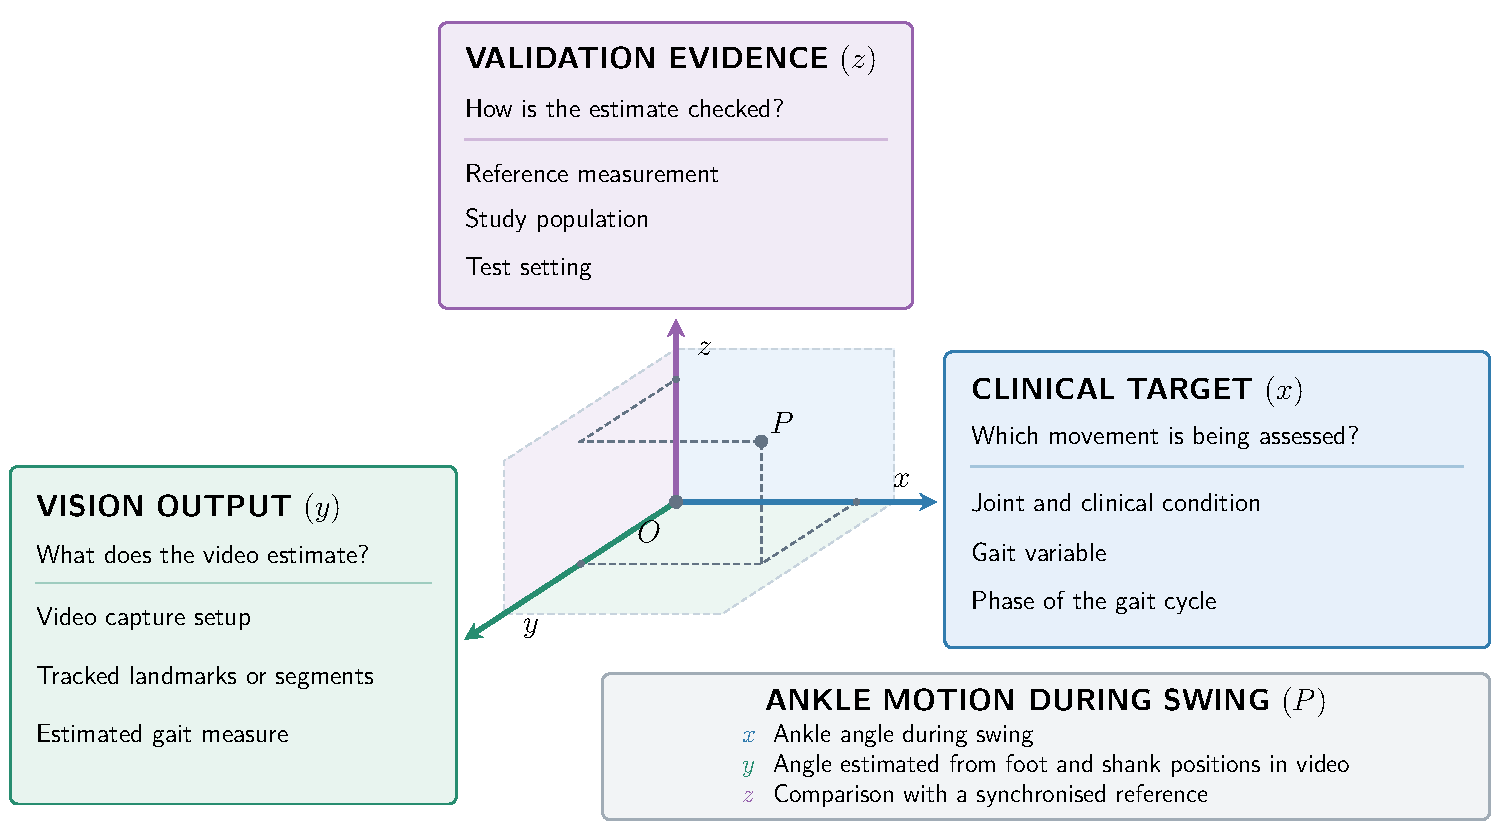
\includegraphics[width=0.75\linewidth]{Images/Figure_02_Gait_Review_Axes.pdf}
    \caption{Three qualitative dimensions of a joint mobility claim. The dashed guides project the ankle-swing example \(P\) onto the clinical target, vision output and validation evidence axes.}
    \label{fig:reviewaxes}
\end{figure}

%\input{Review_Dimensions}

\begin{table}[!htbp]
\centering\small
\caption{\revred{Research questions and where they are addressed.}}
\label{tab:review_questions}
\color{RevisionRed}\hypersetup{allcolors=RevisionRed}
\renewcommand{\arraystretch}{1.09}
\begin{tabularx}{0.98\linewidth}{@{}p{0.10\linewidth}>{\raggedright\arraybackslash}X p{0.19\linewidth}@{}}
\toprule
\textbf{ID} & \textbf{Review question} & \textbf{Sections} \\
\midrule
RQ1 & Which changes in walking are associated with hip, knee and ankle mobility problems, including compensation at adjacent joints? & \ref{sec:JMP} and \ref{sec:JMPWTCV} \\ \addlinespace[3pt]
RQ2 & How do vision-based approaches use pose, gait features and action recognition to measure movement or identify gait patterns? & \ref{sec:JMPCV} and \ref{sec:JMPWCV} \\ \addlinespace[3pt]
RQ3 & What reference measurements, clinical labels and evaluation designs support claims about movement, severity or change over time? & \ref{sec:JMPWTCV}, \ref{sec:KO} and \ref{sec:discussion} \\ \addlinespace[3pt]
RQ4 & How do the recording conditions and the study population limit the use of video-based gait estimates in practice? & \ref{sec:recording_robustness} and \ref{sec:discussion} \\
\bottomrule
\end{tabularx}
\end{table}

\subsection{\revred{Sources and Search Window}}
\label{sec:search_sources}
\begin{redrevision}
We searched IEEE Xplore, the ACM Digital Library, Springer and ScienceDirect. Together, these sources cover technical work on vision and movement analysis and clinical work on gait and rehabilitation (Table~\ref{tab:review_sources}). The search considered English-language peer-reviewed journal and conference papers published through April 2026. 
\end{redrevision}

\begin{table}[!htbp]
\centering\small
\caption{\revred{Sources searched and their relevance to the review. Coverage overlaps across sources.}}
\label{tab:review_sources}
\color{RevisionRed}
\renewcommand{\arraystretch}{1.07}
\begin{tabularx}{0.98\linewidth}{@{}p{0.26\linewidth}>{\raggedright\arraybackslash}X@{}}
\toprule
\textbf{Source} & \textbf{Relevant coverage} \\
\midrule
IEEE Xplore & Computer vision, sensing and engineering approaches to gait and pose estimation. \\
ACM Digital Library & Computer vision and human movement representation, including activity recognition. \\
Springer & Vision methods, movement assessment and rehabilitation research. \\
ScienceDirect & Clinical gait, biomechanics, rehabilitation and applied vision methods. \\
\bottomrule
\end{tabularx}
\end{table}

\subsection{\revred{Search Keys and Fields}}
\label{sec:search_fields}
\begin{redrevision}
The recorded search terms combine clinical expressions such as \emph{joint mobility} and \emph{rehabilitation} with technical expressions such as \emph{markerless gait analysis} and \emph{human pose estimation}. Titles and abstracts were used to check topical relevance. The available search record identifies the terms and sources but leaves the platform-specific query strings and field settings unspecified.
\end{redrevision}

\subsection{\revred{Concept Groups and Query Construction}}
\label{sec:search_concepts}
\begin{redrevision}
Table~\ref{tab:search_concepts} groups the recorded terms by gait, clinical scope and vision method. A clinical search can combine gait and joint terms to find studies that define relevant variables, including work using instrumented measurements. A vision search can combine gait and technical terms, with lower-limb relevance checked at screening. For example, \emph{gait analysis AND (hip OR knee OR ankle) AND (computer vision OR human pose estimation)} illustrates a targeted search. These examples describe the search concepts and help readers plan a follow-up search.
\end{redrevision}

\begin{table}[!htbp]
\centering\small
\caption{\revred{Search concept groups and examples of the recorded terms. The illustrative combinations in the text describe the search logic.}}
\label{tab:search_concepts}
\color{RevisionRed}
\renewcommand{\arraystretch}{1.08}
\begin{tabularx}{0.98\linewidth}{@{}p{0.26\linewidth}>{\raggedright\arraybackslash}X@{}}
\toprule
\textbf{Concept group} & \textbf{Example terms} \\
\midrule
Gait and movement & \emph{gait analysis} \\
Joint and clinical setting & \emph{joint mobility}, hip, knee, ankle, rehabilitation \\
Vision and analysis method & \emph{computer vision}, \emph{markerless gait analysis}, \emph{human pose estimation}, \emph{human action recognition}, \emph{deep learning} \\
\bottomrule
\end{tabularx}
\end{table}

\subsection{\revred{Inclusion and Exclusion Criteria}}
\label{sec:eligibility}
\begin{redrevision}
Studies entered the synthesis through clinical relevance or through an evaluated method for lower-limb gait or joint motion. The outcome and publication requirements in Table~\ref{tab:eligibility} applied to both routes. Studies of general pose estimation, related surveys and work on surface electromyography inform the technical or clinical context where relevant.
\end{redrevision}

\begin{table}[!htbp]
\centering\small
\caption{\revred{Eligibility rules for study selection.}}
\label{tab:eligibility}
\color{RevisionRed}
\renewcommand{\arraystretch}{1.11}
\begin{tabularx}{0.98\linewidth}{@{}p{0.17\linewidth}>{\raggedright\arraybackslash}X >{\raggedright\arraybackslash}X@{}}
\toprule
\textbf{Criterion} & \textbf{Include} & \textbf{Exclude} \\
\midrule
Scope & Clinical work on hip, knee or ankle mobility, or an evaluated approach applicable to lower-limb gait or joint motion. & Unrelated tasks or populations, including identity recognition without a method transferable to lower-limb assessment. \\ \addlinespace[3pt]
Outcome & A gait, biomechanical or functional outcome in a clinical study, or a relevant technical evaluation in a methods study. & Reports without a relevant outcome or evaluation. \\ \addlinespace[3pt]
Publication & A peer-reviewed journal or conference paper in English, published through April 2026. & Outside the language, date or publication criteria, including conference abstracts and editorials. \\ \addlinespace[3pt]
Access and duplication & An available full text and one record per report. & Unavailable full text and duplicate records. \\
\bottomrule
\end{tabularx}
\end{table}

\begin{figure}[H]
\centering
\begin{tikzpicture}[
  stage/.style={
    draw=black!45, fill=black!2, rounded corners=2pt, text=RevisionRed,
    text width=8.3cm, align=left, inner xsep=8pt, inner ysep=6pt, font=\small
  },
  excluded/.style={
    draw=black!45, fill=RevisionRed!5, rounded corners=2pt, text=RevisionRed,
    text width=5.65cm, align=left, inner xsep=7pt, inner ysep=6pt, font=\small
  },
  next/.style={-{Stealth[length=2mm]}, semithick, draw=black!70}
]
\node[stage] (identification) {
  \textbf{Identification}\\
  Search IEEE Xplore, the ACM Digital Library, Springer and ScienceDirect for clinical gait and vision studies.
};
\node[stage, below=4.5mm of identification] (deduplication) {
  \textbf{Filtering}\\
  Match duplicate records and retain one record per report.
};
\node[excluded, right=8mm of deduplication] (duplicates) {
  \textbf{Removed before screening}\\
  Duplicate records.
};
\node[stage, below=4.5mm of deduplication] (screening) {
  \textbf{Title and abstract screening}\\
  Retain reports about hip, knee or ankle mobility, or an approach relevant to assessing lower-limb gait or joint motion.
};
\node[excluded, right=8mm of screening] (offtopic) {
  \textbf{Excluded at screening}\\
  Unrelated tasks or populations outside scope. Biometric studies with no transferable lower-limb method.
};
\node[stage, below=5.5mm of screening] (eligibility) {
  \textbf{Full-text eligibility}\\
  Check for a peer-reviewed journal or conference paper published in English by April 2026. Require a relevant gait, biomechanical or functional outcome, or an evaluated lower-limb method.
};
\node[excluded, right=8mm of eligibility] (ineligible) {
  \textbf{Excluded at eligibility}\\
  Full text unavailable, ineligible date, language or publication type (e.g., abstract or editorial), or no relevant outcome or evaluation.
};
\node[stage, fill=RevisionRed!3, below=4.5mm of eligibility] (included) {
  \textbf{Included in the narrative synthesis}\\
  Clinical and instrumented studies of joint mobility, and evaluated computer-vision methods relevant to gait or joint motion.
};
\draw[next] (identification.south) -- (deduplication.north);
\draw[next] (deduplication.south) -- (screening.north);
\draw[next] (screening.south) -- (eligibility.north);
\draw[next] (eligibility.south) -- (included.north);
\draw[next] (deduplication.east) -- (duplicates.west);
\draw[next] (screening.east) -- (offtopic.west);
\draw[next] (eligibility.east) -- (ineligible.west);
\end{tikzpicture}
\caption{\revred{Screening and selection of studies for the narrative synthesis. The branches show where duplicate, out-of-scope or ineligible records were removed.}}
\label{fig:screening}
\end{figure}


\subsection{\revred{Screening and Selection Procedure}}
\label{sec:screening}
\begin{redrevision}
We removed duplicate records before screening titles and abstracts for relevance. The available full texts were then assessed against the eligibility rules. Figure~\ref{fig:screening} shows the decisions at each stage. It presents the selection rules because database exports and counts for the individual stages were unavailable for reconstruction.
\end{redrevision}



\subsection{\revred{Classification of the Literature}}
\label{sec:classification}
\begin{redrevision}
Figure~\ref{joint_mobility_taxonomy} shows the two evidence groups used in the synthesis. Clinical and instrumented studies help identify the gait variables that matter for hip, knee and ankle mobility. The computer vision studies are discussed by task, including action recognition, video gait analysis and pose estimation. We consider whether a study tests a method on a gait measure or clinical outcome, or whether it provides a technique that could be transferred to joint assessment.

Across both groups, we compare the joint and gait variable, the participant group, recording setup, method, outcome and validation setting. Where a study uses a reference measure or clinical label, we consider what that comparison supports. Agreement with motion capture provides evidence about the accuracy of an angle under the conditions tested. Clinical labels and an appropriate patient sample are needed for a claim about a disorder or its severity. Section~\ref{sec:KO} brings these distinctions together.
\end{redrevision}

\begin{figure}[!htbp]
\centering
\begin{tikzpicture}[level distance=1.5in, sibling distance=.25in, scale=0.7]
\tikzset{
    edge from parent/.style={thick, draw, edge from parent fork right},
    every tree node/.style={draw, minimum width=0.5in, text width=1in, align=center},
    grow'=right
}
\Tree 
[.{Joint Mobility Problems} 
    [.{\rev{Clinical and}\\ \rev{instrumented}}
        [.{Hip Joint} 
            [.\cite{kiss2010effect,shakoor2003asymmetric,ismailidis2021kinematic,laroche2014classification,meyer2015biomechanical,reininga2012subjects,eitzen2012sagittal,mont2007gait} ]
        ]
        [.{Knee Joint} 
            [.\cite{simonsen2012gait,bejek2006influence,kiss2011effect,elbaz2014novel,bacon2022relation,qingguang2015gait,ro2019effects,butler2009gait,harding2012body,da2012biomechanical,kaufman2001gait,weidow2006hip,favre2016gait,phinyomark2016gender,bkaczkowicz2018gait,astephen2008biomechanical,mcclelland2007gait} ]
        ]
        [.{Ankle Joint} 
            [.\cite{reilly2009role,valderrabano2007gait,schmitt2015effect} ]
        ]
    ]
    [.{\rev{Markerless}\\ \rev{computer vision}}
        [.{Human Action\\ Recognition}
            [.\cite{rohan2020human,vemulapalli2014human,li2010action,boswell2021neural,vafadar2021novel,caetano2019skeleton,suhendar2022skeletal,yadav2022skeleton,ke2017skeletonnet,wang2012mining,ahad2021action,uddin2011human,du2015hierarchical,ahmad2019action} ]
        ]
        [.{Gait Analysis\\ using CV} 
            [.\cite{lv2022analysis,ju1996cardboard,leightley2016automated,fan2020gaitpart,cotton2022transforming,prakash2018vision,uccheddu2022rgb,armstrong2022novel,juri2020characterization,ong2017efficacy,blasco2024computer,wang2024markerless,stenum2024clinical,schoenwether2025reliability} ]
        ]
        [.{Human Pose\\ Estimation} 
            [.\cite{ma2022wushu,li2020human,sharma2022surya,viswakumar2019human,stenum2021two,van2023accuracy,sheu2023improvement,marusic2023evaluating,doong2025predicting,yan2025efficient} ]
        ]
    ]
]
\end{tikzpicture}
\caption{\revred{Classification of the clinical and computer vision literature. The citations give examples of each group. Section~\ref{sec:KO} distinguishes clinical validation from evidence about transferable methods.}}
\label{joint_mobility_taxonomy}
\end{figure}


\subsection{\revred{Supporting Material and Traceability}}
\label{sec:supplement_traceability}
\begin{redrevision}
Supplementary Material S1--S3 gives the individual hip, knee and ankle studies. Sections S4--S6 describe the action recognition, video gait and pose estimation studies, and S7 gives the extended method and benchmark comparisons. The tables retain each study's population, setup, outcome and reported result where available. Results can thus be traced to their original study and interpreted in light of its design.
\end{redrevision}

